% !TEX root = ../entropy.tex

\section{Spending profiles predict emergency savings}%
\label{sec:results}

Table~\ref{tab:main} shows the effect of entropy on the probability of building
emergency savings in a given month. Columns (1)-(3) show results for unsmoothed
entropy based on 9 categories, 48 categories, and merchant names, respectively.
Columns (4)-(6) show results for smoothed entropy based on the same variables.
All models include user and year-month fixed effects, and standard errors are
clustered at the user-level. 95\% confidence intervals are shown in
brackets.\footnote{In line with an emerging consensus for how to avoid
    over-reliance on statistical significance, we deliberately do not show
    significance stars in our regression tables and instead emphasise the
    implications of the bounds of the confidence intervals when discussing our
    results. For two recent discussions, see \citet{imbens2021statistical,
romer2020praise}.}

Results for unsmoothed entropy suggest that a one standard-deviation increase
in spending entropy is associated with an increase in the probability of a user
making at least one transfer into their savings accounts of between 1.1 and 2.3
percentage points -- an effect equal to an increase in monthly income of
between \pounds1000 and \pounds2000. Combined, the results in the three columns
present very strong evidence that entropy captures something about users's
spending distribution that is related to their likelihood for making payments
into their savings accounts. Furthermore, entropy variables defined based on a
larger number of unique categories, that allow for a more precise segmentation
of spending behaviour, capture features of spending behaviour that are as
strongly or more strongly related to savings behaviour as monthly income.

The results for smoothed entropy are similar but a tend to be smaller in
magnitude, and -- together -- also provide strong evidence that smoothed
entropy captures features of spending behaviour that is related to savings
behaviour in a statistically significant and economically relevant way. The
main difference to the results for unsmoothed entropy is the reversal of the
sign of the coefficients: across all three measures, an increase in entropy is
estimated to be associated with a decrease in the likelihood of any savings
transactions. The effect of the measure based on 9 categories is not
meaningfully different from zero, but the estimates for the measures based on
48 categories and merchants are almost identical and suggest that the magnitude
of the effect is between 1.2 and 2.1 percentage points -- equalling the effect
of a reduction of monthly income of between \pounds1000 and \pounds2000.

\begin{landscape}
    \begin{table}[ht]
        \centering\scriptsize
        \caption{Effect of entropy on P(savings transactions)}
        \label{tab:main}
        
\begin{table}[htbp]
   \centering
   \tiny
   \begin{threeparttable}[b]
      \caption{\label{tab:reg_has_inflows_main} Effect of entropy on P(transfer into savings accounts)}
      \begin{tabular}{lcccccc}
         \tabularnewline \midrule \midrule
         Model:                     & (1)             & (2)             & (3)             & (4)              & (5)              & (6)\\  
         \midrule
         \emph{Variables}\\
         Entropy (9 cats)           & 0.016$^{***}$   &                 &                 &                  &                  &   \\   
                                    & [0.013; 0.019]  &                 &                 &                  &                  &   \\   
         Entropy (48 cats)          &                 & 0.029$^{***}$   &                 &                  &                  &   \\   
                                    &                 & [0.025; 0.033]  &                 &                  &                  &   \\   
         Entropy (merchant)         &                 &                 & 0.032$^{***}$   &                  &                  &   \\   
                                    &                 &                 & [0.029; 0.036]  &                  &                  &   \\   
         Entropy (9 cats, smooth)   &                 &                 &                 & -0.008$^{***}$   &                  &   \\   
                                    &                 &                 &                 & [-0.010; -0.006] &                  &   \\   
         Entropy (48 cats, smooth)  &                 &                 &                 &                  & -0.023$^{***}$   &   \\   
                                    &                 &                 &                 &                  & [-0.025; -0.020] &   \\   
         Entropy (merchant, smooth) &                 &                 &                 &                  &                  & -0.019$^{***}$\\   
                                    &                 &                 &                 &                  &                  & [-0.021; -0.016]\\   
         Month spend                & 0.009$^{***}$   & 0.009$^{***}$   & 0.008$^{***}$   & 0.009$^{***}$    & 0.008$^{***}$    & 0.007$^{***}$\\   
                                    & [0.009; 0.010]  & [0.008; 0.009]  & [0.008; 0.009]  & [0.009; 0.010]   & [0.007; 0.009]   & [0.007; 0.008]\\   
         Month income               & 0.012$^{***}$   & 0.012$^{***}$   & 0.012$^{***}$   & 0.012$^{***}$    & 0.011$^{***}$    & 0.011$^{***}$\\   
                                    & [0.011; 0.013]  & [0.011; 0.013]  & [0.011; 0.013]  & [0.011; 0.013]   & [0.011; 0.012]   & [0.010; 0.012]\\   
         Has income in month        & 0.086$^{***}$   & 0.084$^{***}$   & 0.083$^{***}$   & 0.087$^{***}$    & 0.085$^{***}$    & 0.086$^{***}$\\   
                                    & [0.077; 0.094]  & [0.075; 0.092]  & [0.074; 0.091]  & [0.079; 0.096]   & [0.076; 0.093]   & [0.078; 0.095]\\   
         Income variability         & 0.001$^{*}$     & 0.001$^{*}$     & 0.001$^{*}$     & 0.001$^{*}$      & 0.001$^{*}$      & 0.000\\   
                                    & [-0.000; 0.001] & [-0.000; 0.001] & [-0.000; 0.001] & [-0.000; 0.001]  & [-0.000; 0.001]  & [-0.000; 0.001]\\   
         \midrule
         \emph{Fixed-effects}\\
         User                       & Yes             & Yes             & Yes             & Yes              & Yes              & Yes\\  
         Year-month                 & Yes             & Yes             & Yes             & Yes              & Yes              & Yes\\  
         \midrule
         \emph{Fit statistics}\\
         Observations               & 1,043,727       & 1,043,727       & 1,043,416       & 1,043,727        & 1,043,727        & 1,043,416\\  
         R$^2$                      & 0.45368         & 0.45395         & 0.45410         & 0.45363          & 0.45415          & 0.45410\\  
         Within R$^2$               & 0.00719         & 0.00768         & 0.00807         & 0.00709          & 0.00805          & 0.00808\\  
         \midrule \midrule
         \multicolumn{7}{l}{\emph{Clustered (User) co-variance matrix, 95\% confidence intervals in brackets}}\\
         \multicolumn{7}{l}{\emph{Signif. Codes: ***: 0.01, **: 0.05, *: 0.1}}\\
      \end{tabular}
   \end{threeparttable}
\end{table}



        \tabnote{1.2\textwidth}{Results from estimating
            Equation~\ref{equ:model}. The
                dependent variable in all columns is a dummy variable
                indicating whether a
                    user made at least one transaction into any of their
                    savings accounts in a
                given period. \regtabinfo}
    \end{table}
\end{landscape}

As discussed in Section~\ref{sub:estimation}, these results are not due to
reverse causality. While we might think that making a savings transactions
might change some or all of the components of entropy discussed in
Section~\ref{sub:spending_profiles} -- the number of unique spending categories
with positive frequency count, the standard deviation of these counts, and the
total number of spend transactions -- and thus change entropy, this is not the
case because of the way we define entropy and savings, and the way spending
transactions are categorised. We define entropy based on all current account
debits that are identified as spends, while we define savings transactions as
the sum of all savings accounts credits. If a user transfers money from their
current account to their savings account, this will be identified as a savings
transaction, but be identified as a transfer on their current account and thus
not considered when calculating their entropy score.

The estimates of our control variables are largely as expected, with the
exception of monthly spend, which one might have expected to be negatively
correlated with savings. Also, it is evident that the strongest predictor among
the included controls for whether a user makes any savings transfer is whether
they receive any income in that month. Income variability, in contrast, is not
correlated with savings behaviour in any economically significant way,
suggesting that people with variable incomes do not build savings cushions for
periods where they have no income.

Overall, the effect of entropy in spending profiles is statistically and
economically significant, and robust across different definitions. In other
words, the scores seem to pick up a feature of the spending distribution that
is predictive of savings behaviour. The obvious question raised by the results
is why smoothing entropy scores flips the direction of the effect of entropy.
We address this next.


\subsection{Why does smoothing flip the direction of the effect}%
\label{sub:why_does_smoothing_flip_the_direction_of_the_effect}

One way to think about the sign change in Table~\ref{tab:main} is to realise
that it implies that at least for some individuals, the relative rank of
smoothed and unsmoothed entropy must differ considerably -- there must be some
individuals that have low unsmoothed entropy but high smoothed entropy or some
that have high unsmoothed entropy and low smoothed entropy or both.
Understanding who those individuals are might thus help us understand the sign
flip.

To understand rank differences between unsmoothed and smoothed entropy scores
it is useful to rewrite Equation~\ref{equ:entropy} in a way that makes it easy
to see its component parts. Remember from Section~\ref{sub:spending_profiles}
that $f_c$ is the number of transactions made by a user in a given period in
spending category $c$, $\setc$ the set of all spending categories, and $F$ the
total number of transactions made by a given user in a given period.
Additionally, let $\setcp = \{c: f_c > 0\}$ be the set of all spending
categories with positive frequency counts (i.e.  with at least one transaction)
and $\setcz = \{c: f_c = 0\}$ the set of all spending categories with a zero
frequency count, so that $\setc = \setcz \cup \setcp$. Then, using our
definitions of unsmoothed and smoothed probabilities, we can write unsmoothed
entropy as

\begin{equation}
\label{equ:entropy_us}
H = -\sum_{c \in \setcp}{\left(\frac{f_c}{F}\right)
log\left(\frac{f_c}{F}\right)},
\end{equation}

and smoothed entropy as:

\begin{equation}
\label{equ:entropy_s}
H^s = -\sum_{c \in \setcp}{\left(\frac{f_c + 1}{F + |\setc|}\right)
log\left(\frac{f_c + 1}{F + |\setc|}\right)}
- |\setcz|\left(\frac{1}{F + |\setc|}\right)
log\left(\frac{1}{F + |\setc|}\right),
\end{equation}

\noindent where the size of set $\setcz$, $|\setcz|$, is the number of all
spending categories in which a user makes no transactions in the period.
These expressions make clear that, by definition, unsmoothed entropy is a
function of frequency counts of categories with positive counts only while
smoothed entropy has two parts: the sum over all additively smoothed frequency
counts of categories with positive counts, plus the same sum for additively
smoothed probabilities of categories with zero counts, which reduces to a
constant term that is multiplied by the number of such categories.

The expressions also make transparent the three main components of both types
of entropy that are determined by user behaviour. The first is the number of
spending categories with a non-zero frequency count, $|\setcp|$, which
determines the number of elements summed over in Equation~\ref{equ:entropy_us},
and partitions the categories into either contributing to the sum on the left
hand side of Equation~\ref{equ:entropy_s} or -- given that for an exogenously
fixed $|\setc|$, $|\setcz| = |\setc \backslash \setcp|$ -- to the constant term
on the right hand side. The second component is the variation of the frequency
counts, $f_c$, and the third component is the number of total spend
transactions, $F = \sum_{\setc}f_c$. Together, these two elements determine the probabilities
associated with a spend transaction occurring in a given category. The number
of total spending categories, $|\setc|$, also determines smoothed entropy and,
implicitly, also unsmoothed entropy since it ``scales'' the number of
categories with a positive frequency count, $|\setcp|$, as a given number of
spending transactions are categorised into finer or coarser categories. But it
is exogenously given and does not depend on user behaviour.

\begin{figure}[ht]
    \centering 
    \caption{Effect of smoothing on entropy}
    \label{fig:scatter_facets}
    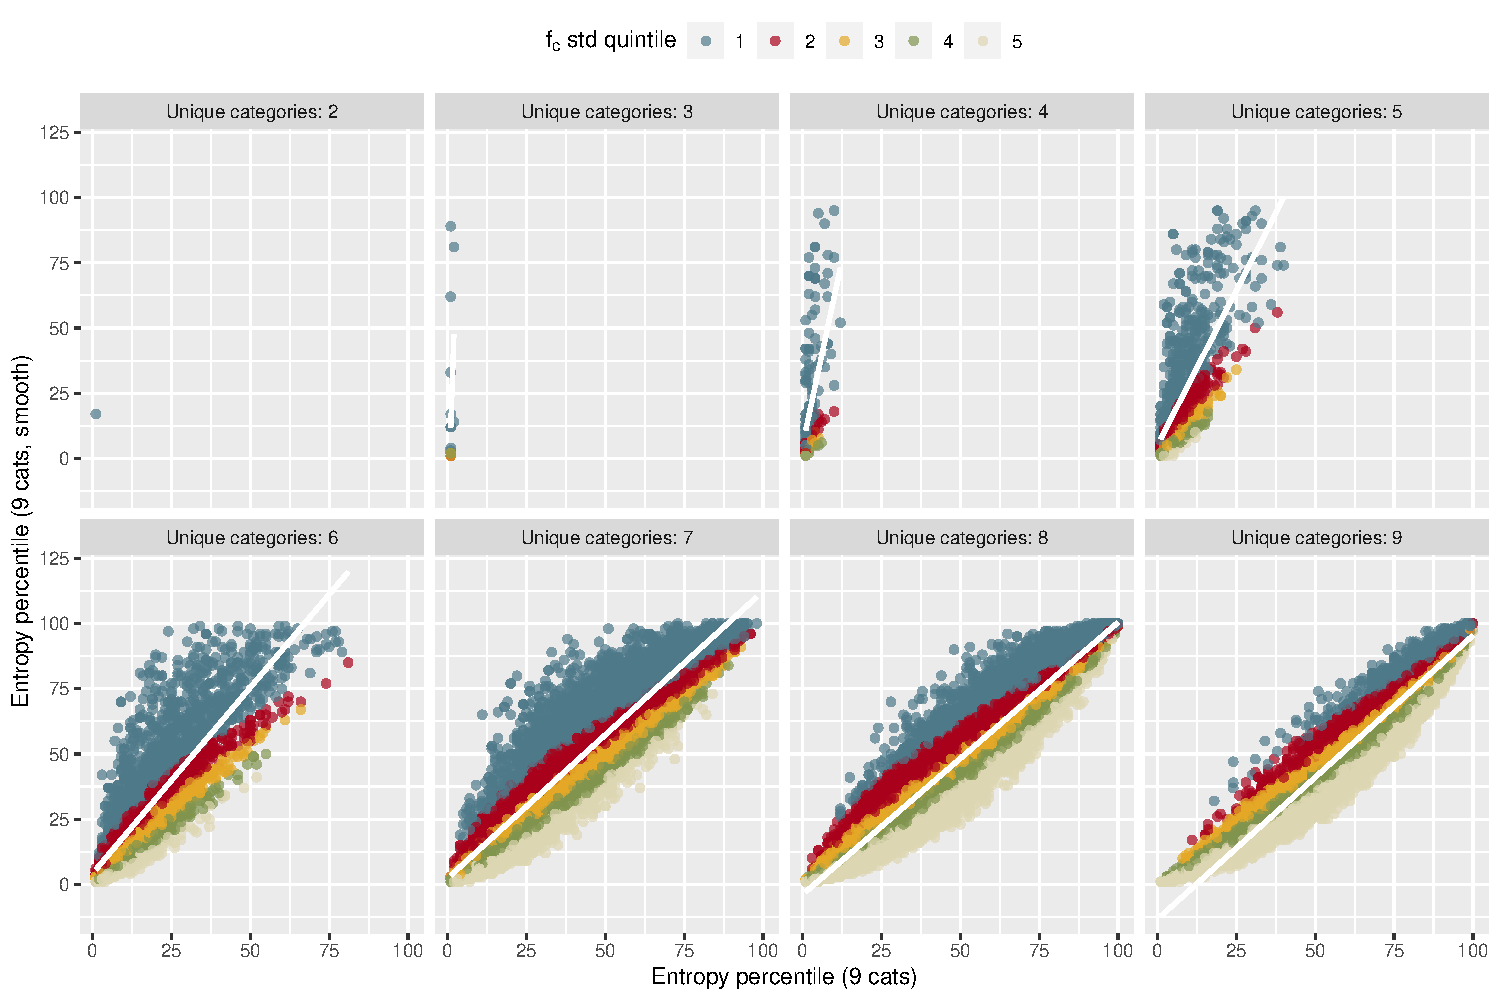
\includegraphics[width=\textwidth]{\figdir/scatter_facet_std_tag_q.pdf}
    \fignote{\textwidth}{Percentile ranks of 9-category-based unsmoothed and
    smoothed entropy separated by the number of categories with positive
frequency counts. White reference lines indicate equal percentile ranks;
colours, frequency count standard deviation quintiles. Figure is based on a
10\% sample of the dataset used for analysis. There are only 8 panels since
there are cases where a user has spends in only a single category.}
\end{figure}

These components help us reason about rank differences between unsmoothed and
smoothed entropy. From equations~\ref{equ:entropy_us} and~\ref{equ:entropy_s}
we can see that the first part of smoothed entropy that sums over all spending
categories with positive frequency counts is very similar to the entire
expression of unsmoothed entropy -- it is that same expression but with
additively smoothed probabilities. Hence, all else equal, the higher the number
of categories with positive counts, the more smoothed entropy is determined by
that first part, and the more similar it will be to unsmoothed entropy. As a
result, we would expect to find large (rank) differences between entropy scores
among cases with few positive-counts categories. Furthermore, given that
unsmoothed entropy is increasing in the number of categories with positive
counts, we expect these cases to have relatively low unsmoothed entropy.

Given that we expect high rank difference cases to make spends across a small
number of categories, and expect these cases to have low unsmoothed entropy,
high rank differences will occur among the subset of those cases that have high
smoothed entropy. Remember from Section~\ref{sub:spending_profiles} that
entropy is higher the more equal the spending category probabilities are.
Hence, for a given number of zero-count categories, smoothed entropy will be
higher if the (additively smoothed) probabilities of all positive-count
categories are close to the (additively smoothed) probabilities of the
zero-count categories, which will be the case (i) if there are few overall
transactions, such that frequency counts ($f_c$) are close to zero and (ii) if
the counts are similar.

Figure~\ref{fig:scatter_facets} visualises this entire line of reasoning for
our 9-category based entropy variable: it shows scatter plots of the percentile
ranks of unsmoothed and smoothed entropy with a reference line indicating
identical rank, separated by the number of categories with positive frequency
counts and coloured based on the quintile of the frequency count standard
deviation.\footnote{Colouring based on the quintile of the total number of
transactions leads to a very similar plot and is thus not shown.} First,
ignoring the colouring and focusing on the shape of the dots only we can see
that, as expected, the relationship between the two entropy measures is tighter
the higher the number of non-zero spending categories is. Cases with large
entropy rank differences are thus to be found among cases with fewer positive
spend categories. Among these, the colouring makes clear that, as expected, the
cases with the largest rank differences -- those with the furthest vertical
difference to the reference line -- have low variation in their frequency
counts. However, it is also clear that the reverse is not true: there are cases
with low count frequency variation that experience little or even a negative
rank difference. Furthermore, among cases with a higher number of categories
with positive counts, cases with a very high variation in frequency counts can
also experience quite large rank differences, albeit in the opposite direction.
Hence, while counts variation is some help in identifying cases with high
entropy rank differences, it does not do so perfectly.

One reason the relationship is not perfect is that while cases with few total
transactions that are evenly spread across a small number of categories will
have high smoothed entropy, such will also have high unsmoothed entropy. What
we are looking for, more precisely, are cases where this pattern holds broadly,
but that also have a small number of frequency counts that dominate the others
but are still relatively close to zero. This would lead to low unsmoothed
entropy (because of the dominant counts) but high smoothed entropy (because all
counts are still relatively close to zero, so that the additively smoothed
distribution resembles a uniform distribution). Further research will be
necessary to more fully classify such cases, and to inquire what it is about
their behaviour that might be related to savings behaviour.


\subsection{Is entropy informative beyond its component parts?}%
\label{sub:is_entropy_informative_beyond_its_component_parts_}

Another question that arises once we think of entropy as comprising three main
component parts is whether its non-linear nature captures anything about the
relationship between spending and saving behaviour that is not captured already
by the three simpler components. 

\begin{landscape}
\begin{table}[ht]
\centering\scriptsize
\caption{Controlling for components}
\label{tab:components}

\begin{table}[htbp]
   \centering
   \tiny
   \begin{threeparttable}[b]
      \caption{\label{tab:reg_has_inflows_comp} Controlling for entropy components}
      \begin{tabular}{lcccc}
         \tabularnewline \midrule \midrule
         Model:                    & (1)             & (2)             & (3)              & (4)\\  
         \midrule
         \emph{Variables}\\
         Entropy (48 cats)         & 0.029$^{***}$   & 0.013$^{***}$   &                  &   \\   
                                   & [0.025; 0.033]  & [0.006; 0.021]  &                  &   \\   
         Entropy (48 cats, smooth) &                 &                 & -0.023$^{***}$   & -0.028$^{***}$\\   
                                   &                 &                 & [-0.025; -0.020] & [-0.034; -0.022]\\   
         Unique categories         &                 & 0.004$^{***}$   &                  & 0.004$^{***}$\\   
                                   &                 & [0.003; 0.005]  &                  & [0.004; 0.005]\\   
         Category counts std.      &                 & 0.002           &                  & -0.015$^{***}$\\   
                                   &                 & [-0.001; 0.006] &                  & [-0.018; -0.011]\\   
         Number of spend txns      &                 & 0.000$^{***}$   &                  & 0.001$^{***}$\\   
                                   &                 & [0.000; 0.001]  &                  & [0.001; 0.001]\\   
         Month spend               & 0.009$^{***}$   & 0.005$^{***}$   & 0.008$^{***}$    & 0.005$^{***}$\\   
                                   & [0.008; 0.009]  & [0.004; 0.006]  & [0.007; 0.009]   & [0.005; 0.006]\\   
         Month income              & 0.012$^{***}$   & 0.011$^{***}$   & 0.011$^{***}$    & 0.011$^{***}$\\   
                                   & [0.011; 0.013]  & [0.010; 0.012]  & [0.011; 0.012]   & [0.010; 0.012]\\   
         Has income in month       & 0.084$^{***}$   & 0.079$^{***}$   & 0.085$^{***}$    & 0.078$^{***}$\\   
                                   & [0.075; 0.092]  & [0.070; 0.087]  & [0.076; 0.093]   & [0.070; 0.087]\\   
         Income variability        & 0.001$^{*}$     & 0.000           & 0.001$^{*}$      & 0.000\\   
                                   & [-0.000; 0.001] & [-0.000; 0.001] & [-0.000; 0.001]  & [-0.000; 0.001]\\   
         \midrule
         \emph{Fixed-effects}\\
         User                      & Yes             & Yes             & Yes              & Yes\\  
         Year-month                & Yes             & Yes             & Yes              & Yes\\  
         \midrule
         \emph{Fit statistics}\\
         Observations              & 1,043,727       & 1,043,727       & 1,043,727        & 1,043,727\\  
         R$^2$                     & 0.45395         & 0.45498         & 0.45415          & 0.45515\\  
         Within R$^2$              & 0.00768         & 0.00956         & 0.00805          & 0.00986\\  
         \midrule \midrule
         \multicolumn{5}{l}{\emph{Clustered (User) co-variance matrix, 95\% confidence intervals in brackets}}\\
         \multicolumn{5}{l}{\emph{Signif. Codes: ***: 0.01, **: 0.05, *: 0.1}}\\
      \end{tabular}
   \end{threeparttable}
\end{table}



\tabnote{1.5\textwidth}{\regtabinfo}
\end{table}
\end{landscape}

We can test this by checking whether the relationship between spending entropy
and the probability of making a savings transaction remains economically and
statistically significant once we control for the three components. Columns (1)
and (3) in Table~\ref{tab:components} replicate the results for the 48-category-based
unsmoothed and smoothed entropy measures presented in Table~\ref{tab:main} for
reference. In columns (2) and (4) we additionally control for the three entropy
components. Including these components has some effect: the coefficients change
slightly -- decreasing in absolute magnitude in the case of unsmoothed entropy,
increasing in the case of smoothed entropy -- while the width of the confidence
intervals about double in both cases, reflecting the strong collinearity amount
the component and entropy. However, both coefficients remain statistically
significant and their confidence intervals cover values that are also
economically significant. Hence, the results make clear that the results in
Table~\ref{tab:main} cannot be attributed simply to the effect of one or more
of entropy's simple components.



